\chapter{Implementation Details}\label{c:implementation}

Our application consists of four concrete parts, the \textit{coordinator}, the data providers, the SMPC cluster and the user interface.

\section{Coordinator}\label{s:impl-coordinator}
The \textit{coordinator} handles all private computation requests, communicates with the data providers -- requesting them to securely import their data to the computing cluster, initiates the secure computation in the SMPC cluster, and finally returns to the user the requested analytics results.

The coordinator server has been designed as a Representational State Transfer (REST) web service.
This design helps decoupling server and client applications; the API that provides is cleaner and easier to understand / discover.
It's standard format / usage makes it easy for new clients to use the application even if the application was not designed with these clients' use cases in mind.

We have implemented this web service using \texttt{Node.js} and more specifically the \texttt{Express server} minimal web framework.

The RESTful API provided by the coordinator server can be found in the following section.


\subsection{RESTful API}\label{ss:coord-restful-api}

\begin{table}[H]
  \centering
  \caption{Coordinator's RESTful API}
  \label{t:coordinator-api}
\begin{tabular}{l}
  \hyperref[s:post1]{
\includegraphics[page=1,width=\textwidth]{figures/post1.pdf}} \\
  \hyperref[s:post2]{
\includegraphics[page=1,width=\textwidth]{figures/post2.pdf}} \\
  \hyperref[s:post3]{
\includegraphics[page=1,width=\textwidth]{figures/post3.pdf}} \\
  \hyperref[s:get1]{
\includegraphics[page=1,width=\textwidth]{figures/get1.pdf}} \\
\end{tabular}
\end{table}


The RESTful API of the \textit{coordinator} is summarized in table \ref{t:coordinator-api}.
The two first POST requests initiate a secure histogram computation for numerical and categorical values respectively.
With the third POST request a user can request a secure decision tree computation for either numerical or categorical values, specifying in the request body one of ID3 and C4.5 classifiers.
The \texttt{/smpc/queue} GET request is for checking the status and/or result of a specified computation request (the aforementioned POST requests).
In appendix \ref{s:coordinator-api} we explain in more detail each individual POST and GET request.


\subsection{Sequence of Actions}\label{ss:coordinator-sequence}

In section \ref{ss:end-to-end-execution-flow} we have presented a brief overview of the end\hyp to\hyp end query execution.
In this section, we elaborate on this brief overview, including many implementation details that have been omitted.

\begin{description}[labelwidth=4em, leftmargin=\dimexpr\labelwidth+\labelsep\relax]
  \item [Step 1:] A user makes a privacy\hyp preserving analytics request to the \textit{coordinator}.

  This request is either made from the UI (presented in section \ref{s:impl-ui}) or from another service (\textit{e.g.} Postman tool\footnote{\href{https://www.getpostman.com}{https://www.getpostman.com}}, or even another custom UI that accords with our API).


  \item [Step 2:] The \textit{coordinator} server is responsible for orchestrating all the involved parties: it communicates with the data\hyp providers requesting secure data\hyp import to the SMPC cluster.
  \begin{enumerate}[label=\subscript{2}]
    \item The \textit{coordinator} maintains a database with the IP addresses of all hospitals involved in the privacy\hyp preserving computation so it can send import requests.
    \item The user has the option to select which of the data providers to involve in the secure computation. The \textit{coordinator} sends import requests to the selected data providers.
    \item After the import procedure has finished, the \textit{coordinator} is responsible to return the results to the user. If the initial request has been made from the UI, the results are visualized and returned through the UI, otherwise a JSON file is returned to the user.
  \end{enumerate}


  \item [Step 3:] The data\hyp providers extract the requested data from their datasets and securely import them to the SMPC cluster applying secret\hyp sharing.

  A database is maintained in each hospital with all its private data.
  However, in each request, the user selects which attributes take part in the privacy\hyp preserving analytics.

  \begin{enumerate}[label=\subscript{3}]
    \item Each hospital's server receives a secure data import request from the \textit{coordinator} for the user selected attributes.
    \item A data extraction and a secret sharing procedure takes place in each hospital's server in order to securely import the data to the SMPC cluster.
  \end{enumerate}

  The data\hyp import procedure is described in more detail in section \ref{ss:data-providers-importer}.


  \item [Step 4:] The SMPC cluster computes the privacy preserving analytics on the requested data and returns the results to the \textit{coordinator}.

  Depending on the user's request, the SMPC cluster execute either a secure aggregation or a secure decision tree algorithm.
  After the computation has finished, the SMPC cluster returns the results to the \textit{coordinator}.


  \item [Step 5:] Finally, the results are returned to the user through the \textit{coordinator}.

  If the initial request has been made from the UI, the results are visualized and returned through the UI, otherwise a JSON file is returned to the user as described in section \ref{ss:coord-restful-api}.

\end{description}



\subsection{Result Caching}\label{ss:caching}
Privacy-preserving algorithms can sometimes be highly time-demanding.
Execution times vary depending on the number of patients, attributes, and also the analytics algorithm that is used.
For instance, by definition, decision trees require way more computational power that aggregators do.
Similarly, their privacy\hyp preserving equivalents are computationally intensive tasks.

Furthermore, since our end-to-end system is designed to accept hundreds of requests per day, it is computationally infeasible to meet them all.
Not to mention, that many of them could possible be the same request -- or even repeated.

For all those reasons, we have implemented a caching mechanism that stores secure computation results so future requests for that data can be served faster.
If a cache hit occurs, the secure computation is omitted and the results are immediately returned to the user.
Otherwise, if a cache miss occurs, the secure computation will normally continue as described in sections \ref{s:architecture} and \ref{ss:coordinator-sequence}.

However, a proficient user may want to omit the already computed results, in case of a recent dataset modification.
In this case, he/she can explicitly specify that the cache should not be used by adding a ``cache'': ``no'' option in the JSON request body.
For the average user, that would not be necessary, since our system invalidate cache results that are older than 1 month.





%%%%%%%%%%%%%%%%%%%%%%%%%%%%%%%%%%%%%%%%%%%%%%%%%%%%%%%%%%%%%%%%%%%%%%%%%%%%%%%%
%%%%%%%%%%%%%%%%%%%%%%%%%%%%%%%%%%%%%%%%%%%%%%%%%%%%%%%%%%%%%%%%%%%%%%%%%%%%%%%%

\section{Data Providers}\label{s:impl-data-providers}
When a private computation request arises, the \textit{coordinator} server communicates with the data providers and requests them to securely import their data to the computing cluster.
Finally the \textit{coordinator} returns the results of the computation to the researcher.

Data providers run their own web server that listen to import requests from the \textit{coordinator}.

That server is implemented using \texttt{Node.js Express Server}, and provides the following RESTful API.


\subsection{RESTful API}\label{ss:data-providers-restful-api}


\begin{table}[H]
  \centering
  \caption{Data Providers' RESTful API}
  \label{t:data-providers-api}
\begin{tabular}{l}
  \hyperref[s:post4]{
\includegraphics[page=1,width=\textwidth]{figures/post4.pdf}} \\
  \hyperref[s:post5]{
\includegraphics[page=1,width=\textwidth]{figures/post5.pdf}} \\
\end{tabular}
\end{table}


The RESTful API of the data providers is summarized in table \ref{t:data-providers-api}.
The above two POST requests initiates a secure import for numerical and categorical datasets respectively.
In appendix \ref{s:data-providers-api} we explain in more detail the two types of POST requests that the \textit{coordinator} sends to the data providers.


\subsection{Data Importer}\label{ss:data-providers-importer}
The secure data import is one of the most essential procedures in the secure multi-party computation scenario.
In this step, the data are secret-shared to the three computing parties.
The shares are cryptographic part of the secret but reveal nothing about it.
In section \ref{s:secret-sharing}, we examined some secret sharing techniques and the homomorphic properties that some of them have.
In simple words, the secret sharing homomorphic property enables meaningful computation on the shares of the initial data.

We use a standard tabular structure for the data in order to import them in the SMPC cluster's encrypted database provided by Sharemind.
The datasets to be imported should be in comma-separated values (CSV) format.
In case that a dataset has some other non-tabular arrangement (see section \ref{c:datasets}), we transform them in the standard CSV format using software that we developed for that particular task.

The aforementioned procedure is described in more detail in section \ref{c:datasets}.




\subsection{Containerization}\label{ss:data-providers-containerization}
The number of data providers can start from just one (trivial case), and grow unrestrictedly.
The case with only one data provider is when that provider just wants to outsource the computation to a cloud, without having to trust an individual server.
The case of multiple data providers is the most common case, where the providers wish to perform computation over the union of all datasets without anyone being able to learn anything more than the computation's output.
Thus, we wanted the deployment of each data provider to be easy and fast; veiling all the individual parts, such as the required packages, the SMPC importer installation, any software for data pre\hyp processing etc.

For that reason we decided that the best choice is to offer a containerized solution. We used Docker\footnote{\href{https://www.docker.com/}{https://www.docker.com/}} for the building and shipping of an \textit{image} with everything installed and ready to run.
That image also includes the web server accepting requests for data import (according to the API specified in section \ref{ss:data-providers-restful-api}), already up and running.

Each individual data provider, can use this image to create a lightweight, portable, self-sufficient container, which can run virtually anywhere.
The container will run locally in the provider's premises.
The only requirement that a data provider has is to upload its datasets to the container in order to be able to securely import them into the SMPC cluster. In this way, non-expert users can easily provide their data to be a part of the secure computation.



%%%%%%%%%%%%%%%%%%%%%%%%%%%%%%%%%%%%%%%%%%%%%%%%%%%%%%%%%%%%%%%%%%%%%%%%%%%%%%%%
%%%%%%%%%%%%%%%%%%%%%%%%%%%%%%%%%%%%%%%%%%%%%%%%%%%%%%%%%%%%%%%%%%%%%%%%%%%%%%%%

\section{SMPC Cluster}\label{s:impl-smpc-cluster}
For the purpose of this dissertation, we have deployed the Sharemind secure computing platform on three 64\hyp bit virtual machines (VM), each running Ubuntu 18.04.
The three VMs share an Intel Xeon E5-2670 (v2) at 2.50 GHz.
Each VM utilizes 6 cores and 8 GB of memory.

As described in section \ref{s:computing-parties-collusion}, ideally, the three computing nodes should be deployed in premises with conflicting interests, preventing any adversary from controlling all of them simultaneously.
This should not be confused with trusted servers.




%%%%%%%%%%%%%%%%%%%%%%%%%%%%%%%%%%%%%%%%%%%%%%%%%%%%%%%%%%%%%%%%%%%%%%%%%%%%%%%%
%%%%%%%%%%%%%%%%%%%%%%%%%%%%%%%%%%%%%%%%%%%%%%%%%%%%%%%%%%%%%%%%%%%%%%%%%%%%%%%%

\section{User Interface}\label{s:impl-ui}
Apart from the RESTful API, a user/researcher can initiate a secure computation through our user interface (UI), deployed in \href{https://mhmd.madgik.di.uoa.gr/}{https://mhmd.madgik.di.uoa.gr/}.
Our the goal was to design a simple and elegant user interface which is easy to use and in the same time enjoyable (user\hyp friendly).


In the landing page, except from reading and understanding useful information about the end\hyp to\hyp end infrastructure, the operator can choose between two options: secure data aggregation and secure data classification, as depicted bellow\footnote{In appendix \ref{c:ui} we have included the whole landing page as a screen\hyp shot, as well as many other components of the UI.}.

\begin{figure}[H]
  \centering
  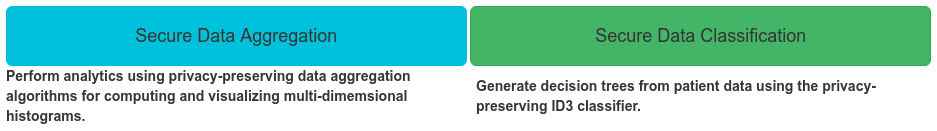
\includegraphics[width=\columnwidth]{figures/landing_buttons.png}
  \caption{Landing page: choosing between secure data aggregation \& classification}
  \label{f:landing-buttons}
\end{figure}

Consecutively, the user can select the desired dataset on which the algorithms will execute, as in figure \ref{f:mesh-cvi}\footnote{The option for selecting dataset for secure classification is identical.}.

\begin{figure}[H]
  \centering
  
\includegraphics[width=\columnwidth]{figures/mesh_cvi.png}
  \caption{Selecting dataset for secure aggregation}
  \label{f:mesh-cvi}
\end{figure}



\textbf{Secure Aggregation for the CVI dataset:} After selecting the secure aggregation for the CVI (numerical) dataset, the researcher has to choose attributes and their corresponding histogram cells ($\beta$ factor), and optionally filters and data\hyp providers for the privacy\hyp preserving computation, as in figure \ref{f:cvi-histogram}.
The results of this computation are shown in figure \ref{f:cvi-histogram-results}.

\begin{figure}[H]
  \centering
  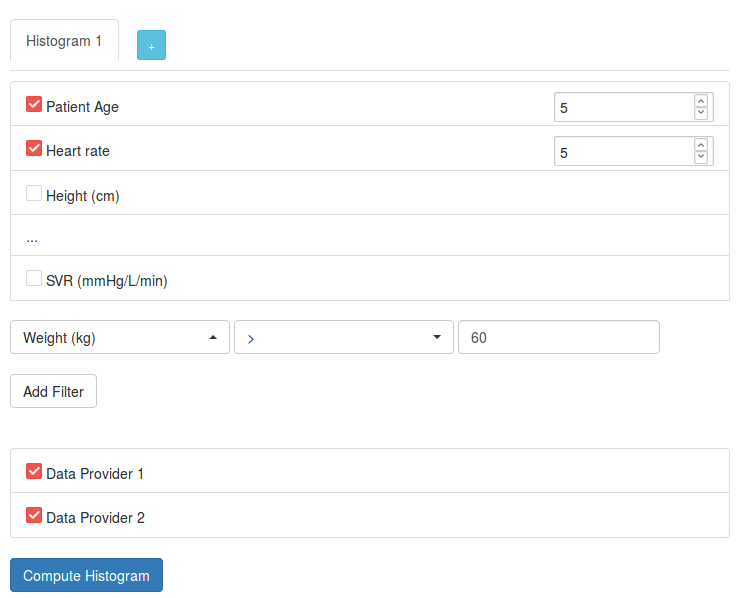
\includegraphics[width=0.8\columnwidth]{figures/cvi_histogram.png}
  \caption{Choosing attributes, filters and data\hyp providers for secure aggregation for numerical dataset}
  \label{f:cvi-histogram}
\end{figure}

\begin{figure}[H]
  \centering
  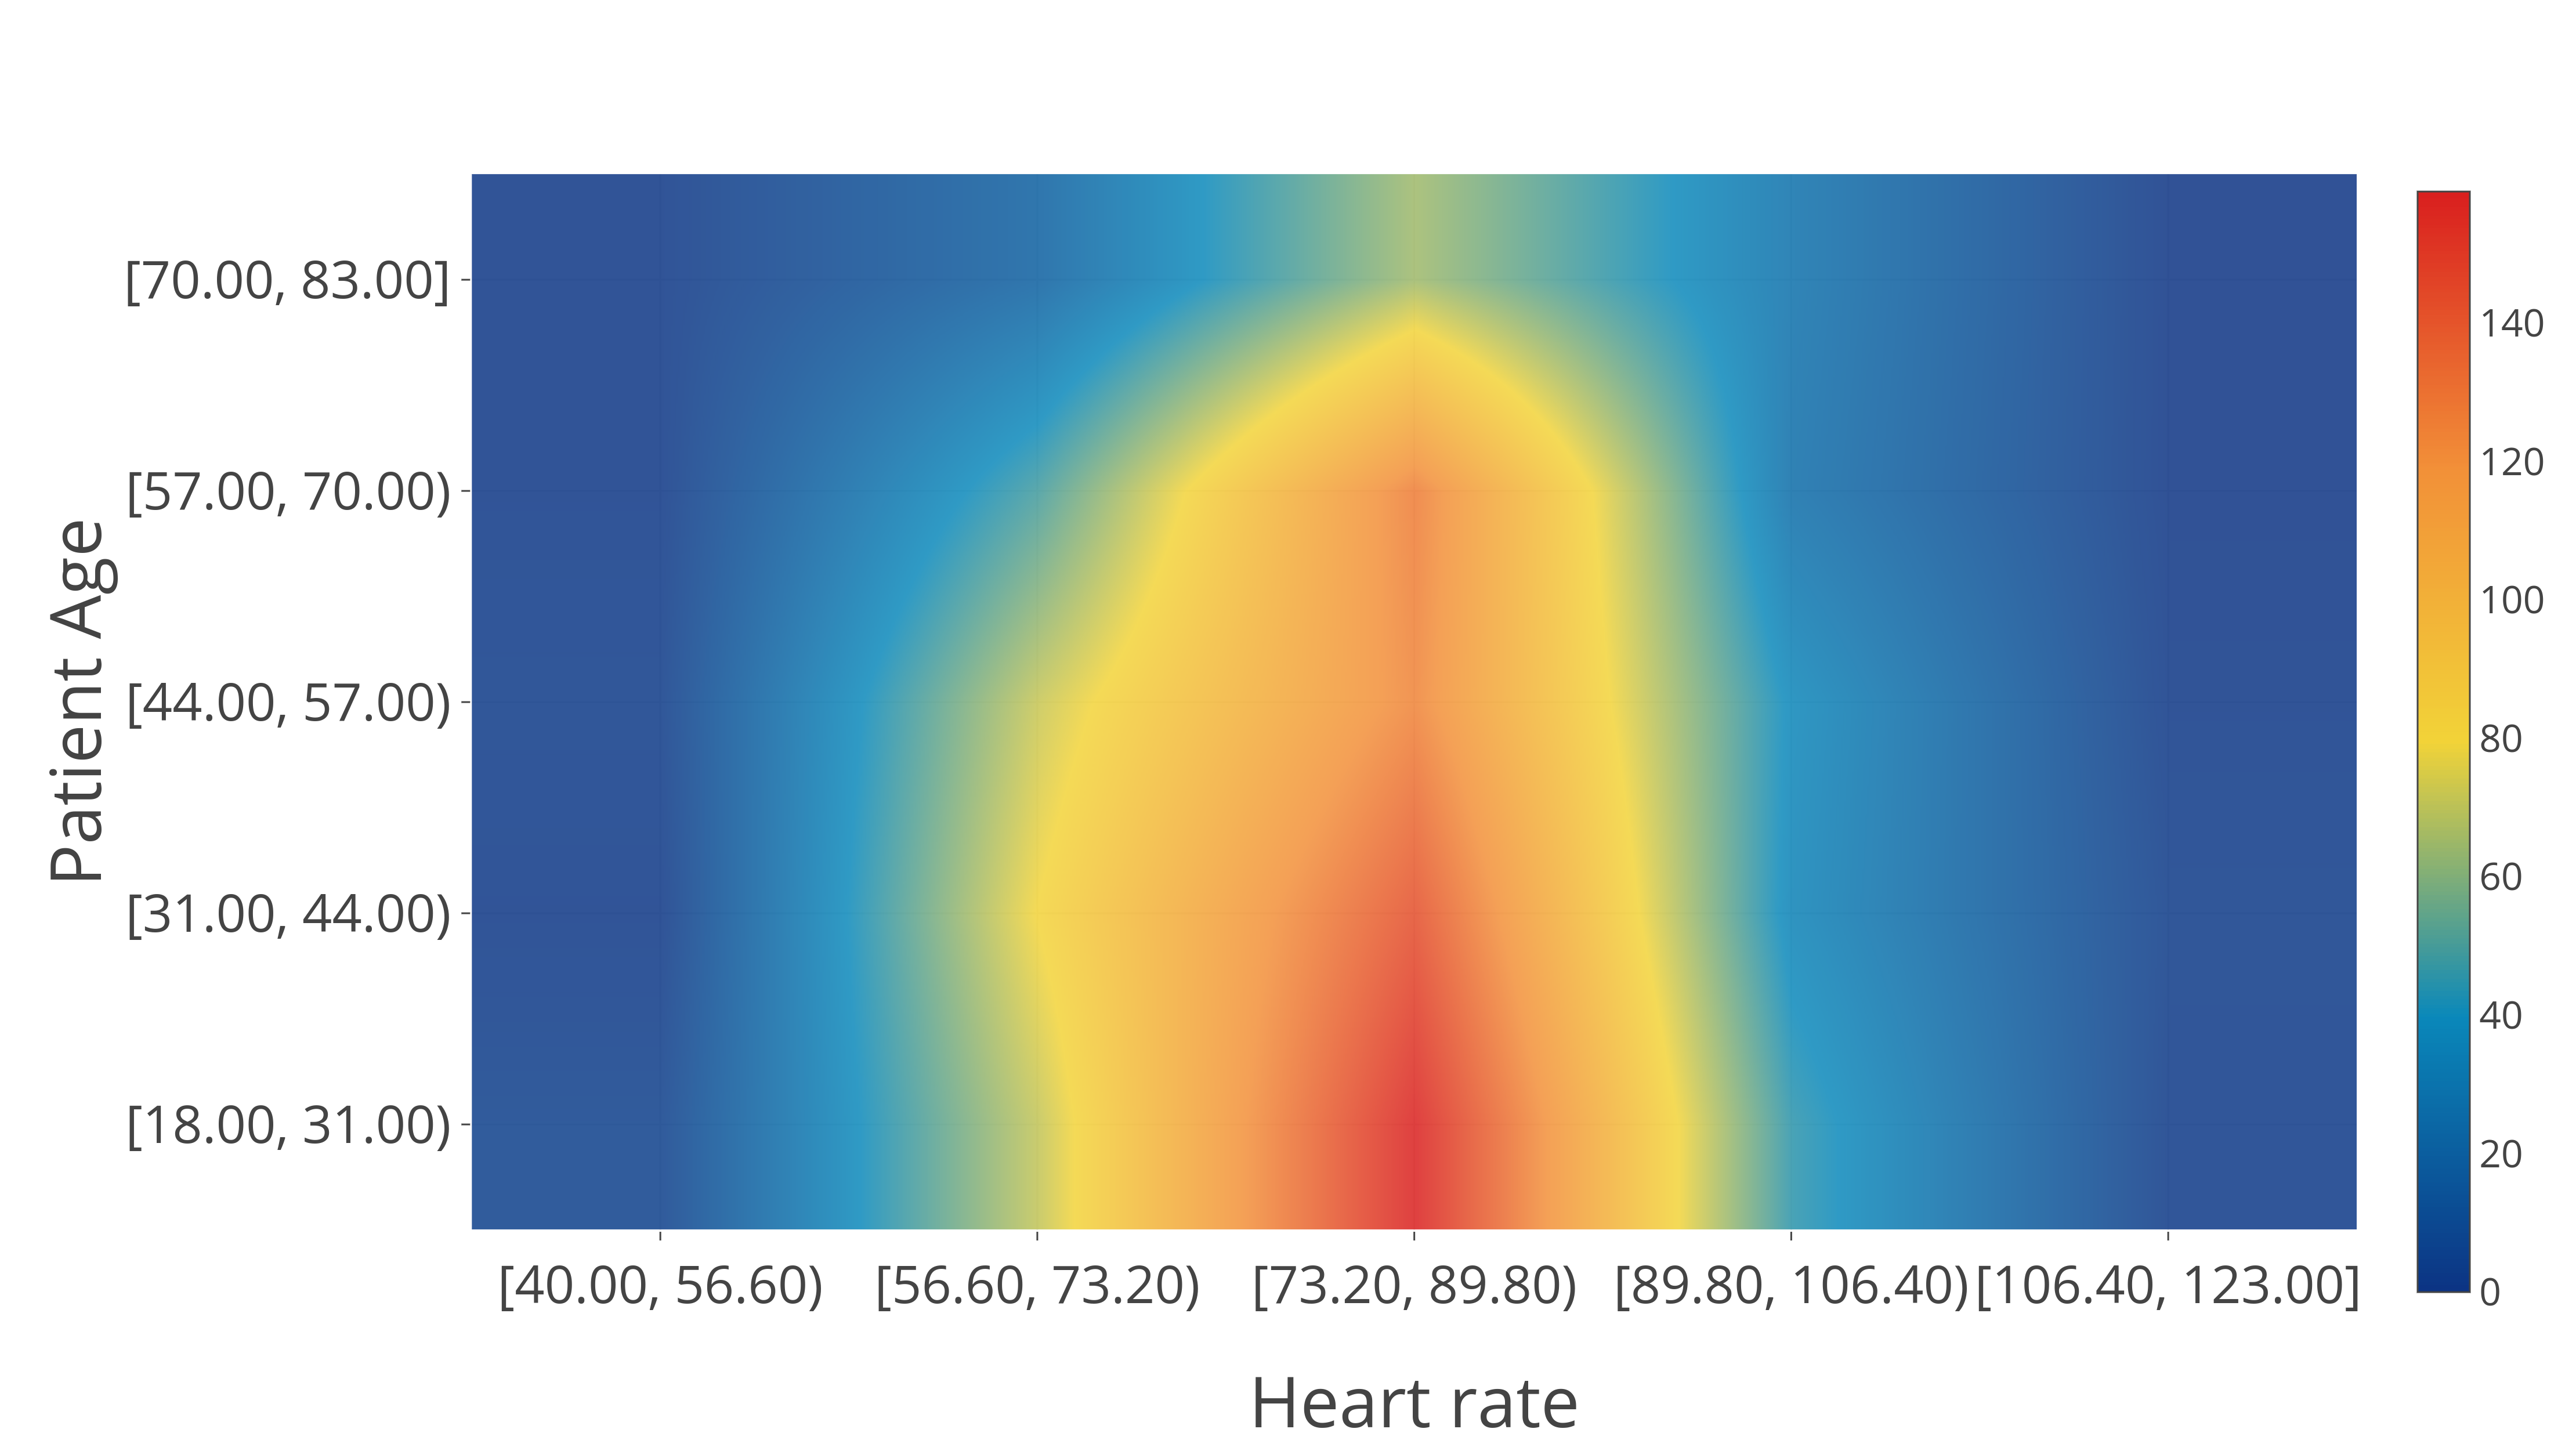
\includegraphics[width=0.8\columnwidth]{figures/cvi_histogram_results.png}
  \caption{2D Histogram for ``Patient Age'' \& ``Heart Rate'' for $\beta = 5$ for each dimension}
  \label{f:cvi-histogram-results}
\end{figure}


\textbf{Secure Aggregation for the MeSH dataset:} After selecting the secure aggregation for the MeSH (categorical) dataset, the researcher has to choose attributes, filters and data\hyp providers for the privacy computation.
For instance, in figure \ref{f:mesh-histogram} the user has specified a 2\hyp dimensional histogram for attributes ``Age Groups [M01.060]'' and ``Population Groups [M01.686]'', filtering the ``Diseases [C]'' attribute in ``Virus Diseases [C02]'' or ``Parasitic Diseases [C03]''.

\begin{figure}[H]
  \centering
  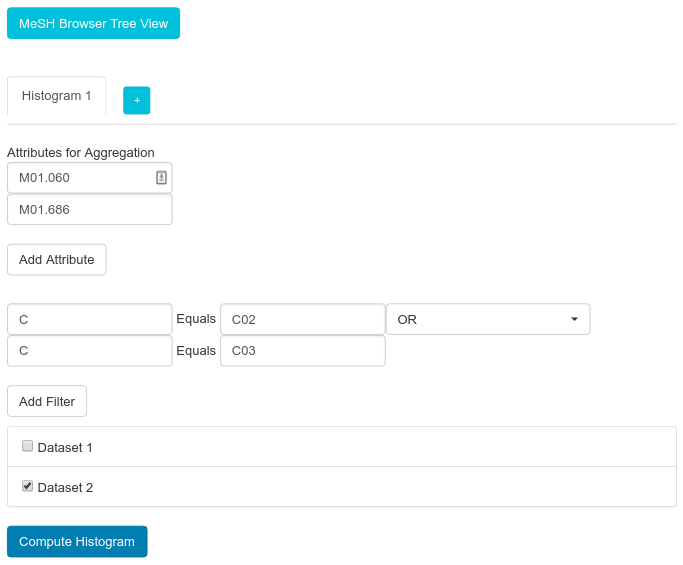
\includegraphics[width=0.8\columnwidth]{figures/mesh_histogram.png}
  \caption{Creating a histogram on the MeSH dataset}
  \label{f:mesh-histogram}
\end{figure}



\textbf{Secure Classification for the CVI dataset:} The UI for secure classification on the CVI dataset is similar to the secure aggregation, however it has two extra entries, one for the \emph{class\hyp attribute} and one for the classification algorithm (currently ID3 or C4.5).

\textbf{Secure Classification for the MeSH dataset:} Finally, the UI for secure classification on the MeSH dataset is similar to the secure aggregation one, having two extra entries as well.


More screenshots are included in appendix \ref{c:ui}.

\fixme{Add more screenshots in appendix!}


\section{Communication}\label{s:impl-communication}
We employ encryption for data in transit using Transport Layer Security (TLS).
All communication through the \textit{coordinator} uses Hypertext Transfer Protocol Secure (HTTPS), with a certificate issued from Let's Encrypt\footnote{https://letsencrypt.org/}.
Thus, all secure computation requests as well as the private\hyp computed results are transferred encrypted.
Also, since HTTPS provides authentication of the accessed website, the users know that they communicate with the correct server.


